\documentclass[10pt,a4paper]{article}

%%%%%%%%%%%%%%%%%%%%%%%%%%%
% MODIFY:

\newcommand{\authorA}{Ahmad Bin Qasim (03693345)}
\newcommand{\authorB}{Kaan Atukalp (03709123)}
\newcommand{\authorC}{Martin Meinel (03710370)}
\newcommand{\groupNumber}{H} % - YOUR GROUP NUMBER
\newcommand{\exerciseNumber}{4} % - THE NUMBER OF THE EXERCISE
\newcommand{\sourceCodeLink}{https://gitlab.lrz.de/ga53rog/praktikum-ml-crowd}

\newcommand{\workPerAuthor}{
\authorA&Task 1&33\%\\
      &Task 2&33\%\\
      &Task 3&33\%\\
      &Task 4&33\%\\
      &Task 5&33\%\\
      \hline
\authorB&Task 1&33\%\\
      &Task 2&33\%\\
      &Task 3&33\%\\
      &Task 4&33\%\\
      &Task 5&33\%\\
      \hline
\authorC&Task 1&33\%\\
      &Task 2&33\%\\
      &Task 3&33\%\\
      &Task 4&33\%\\
      &Task 5&33\%\\
}

%%%%%%%%%%%%%%%%%%%%%%%%%%%

%%
% imports for the exercise sheets
%

\usepackage[utf8]{inputenc}
\usepackage{amsmath}
\usepackage{amsfonts}
\usepackage{amssymb}

\usepackage[yyyymmdd]{datetime}
\renewcommand{\dateseparator}{--}

\usepackage[left=2cm,right=2cm,top=3cm,bottom=3cm]{geometry}

\usepackage{hyperref}

\usepackage{amsthm}
\newtheorem{lem}{Lemma}
\newtheorem{thm}{Theorem}
\newtheorem{cor}{Corollary}
\newtheorem{rem}{Remark}
\newtheorem{definition}{Definition}
\newtheorem{ter}{Terminology}

\usepackage{graphicx}

\newcommand{\M}{\mathcal{M}}
\newcommand{\N}{\mathcal{N}}
\newcommand{\K}{\mathcal{K}}
\newcommand{\SPDk}{\mathbb{P}^k}
\newcommand{\vol}{\text{vol}}

\newcommand{\Figref}[1]{Figure~\ref{#1}}
\newcommand{\figref}[1]{figure~\ref{#1}}
\newcommand{\Eqnref}[1]{Equation~(\eqref{#1})}
\newcommand{\eqnref}[1]{equation~(\eqref{#1})}

\usepackage{float}
\usepackage{tabularx}
\usepackage{subcaption}
\usepackage{mwe}

\usepackage{fancyhdr}
\pagestyle{fancy}

\usepackage{totcount}
\newtotcounter{taskCounter}
\newtotcounter{pointCounter}
\newenvironment{task}[1]{\noindent\stepcounter{taskCounter}\textbf{Report on task #1}\smallbreak\hrule\smallbreak}{\smallbreak\hrule\bigbreak}


\title{Report for exercise \exerciseNumber~from group~\groupNumber}

\makeatletter
\let\thetitle\@title
\let\theauthor\@author
\let\thedate\@date
\makeatother

\providecommand{\versiondate}{\today}

\lhead{Exercise sheet \exerciseNumber}
\chead{Master Praktikum: Modelling and Simulation of Crowds WS2019/20}
\rhead{TUM}
\lfoot{Report of Group \groupNumber}
\cfoot{\thepage}
\rfoot{Last compiled: \versiondate}
\renewcommand{\headrulewidth}{0.4pt}
\renewcommand{\footrulewidth}{0.4pt}

\newcommand{\frontpage}{
\begin{center}
\textbf{\thetitle}\\~\\
\end{center}
\begin{table}[H]
\begin{tabular}{ll}
Tasks addressed:&\total{taskCounter}\\
Authors:&\authorA\\
&\authorB\\
&\authorC\\
Last compiled:&\versiondate\\
Source code:&\sourceCodeLink
\end{tabular}
\end{table}
\vfill
The work on tasks was divided in the following way:
\begin{table}[H]
\begin{tabularx}{\textwidth}{X|p{2cm}|p{2cm}}
\workPerAuthor
\end{tabularx}
\end{table}
\newpage
}

\begin{document}

\frontpage

\begin{task}{1, Principal component analysis}
First part: 

Energy of the two components: 
energy of pc1: 0.9929871280253524 energy of pc2 0.0070128719746476165 

Second Part: 
Rerun it using columns rather than rows 

Third Part: 
They are walking in loops. 
energy of pc1: 0.47330561274983274 energy of pc2 0.3759408098565421 
Total Energy is around 84\%. Two components are enough to capture the most energy. 
It is enough because in comparison to the original plot the reconstructed plot looks similar and still captures the most information. 
\end{task}
\begin{task}{2, Diffusion Maps}
Part 2: 

Energy values:  
pc3 0.28867937283177014  
pc2 0.3292051971173148  
pc1 0.3821154300509151 

The first two Principal components cover only 71.1\% So we would lose 28.9\% of the data.
In comparison to that we can cover almost the whole dataset by taking the first three principal components. Consequently, it makes much more sense to take all principal components instead of two. 
\end{task}
\begin{task}{3, Training a Variational Autoencoder on MNIST}
\begin{enumerate}
	\item We used a linear activation function to approximate the mean and standard deviation of the posterior distribution because, the mean and standard deviation values are unbounded. Other activation functions bound the output value to a certain range. We considered different activation functions but discarded it because of the bounded output. [\ref{tab:activation}]
\begin {table}[H]
\caption {Different activation functions} \label{tab:activation} 
\begin{center}
\begin{tabular}{ | m{10em} | m{10em}| } 
\hline
Activation Function& Bounds \\ 
\hline \hline
Sigmoid & (0,1) \\ 
\hline
Tanh & (-1,1) \\
\hline
Relu & max(0,x) \\
\hline
\end{tabular}
\end{center}
\end{table}
	\item If the reconstructed image are much better then the generated images then, it means that the model has been overfitted to the input data distribution. This can happen when the KL-divergence loss (latent loss) of the approximated posterior distribution does not converge while the reconstruction loss of the input distribution converges. 
	
	In order to solve this problem, the reconstruction loss and the KL-divergence loss can be weighted to give more weight to the latter.
	
	\item After training the Variational Autoencoder model, We plotted the desired graphs. The latent space of the encoder is 2 dimensional. [\ref{fig:latent-2}]. In addition to the configurations provided in the exercise sheet, related to the model, the following changes were made:
	\begin{itemize}
		\item The output of the decoder is not the mean of likelihood but the predicted data points. This modification within the decoder can be considered as probabilistic as well because it is equivalent to modeling likelihood as Gaussian with identity covariance
		\item Binary cross entropy is used to calculated the reconstruction loss with the predicted data points from decoder and the input data as the target.
		\item The last layer of decoder uses a Sigmoid activation as the data in mnist is grayscale. 
	\end{itemize}
	
\begin{figure}[H]
\caption{results obtained with a 2 dimensional latent space}
\label{fig:latent-2} 
\begin{tabular}{cccc}
  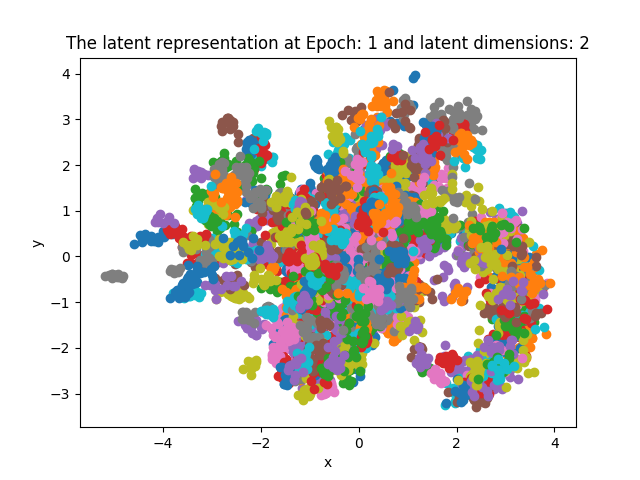
\includegraphics[width=0.23\textwidth]{../plots/task3/latent_epoch1_latent2.png} &   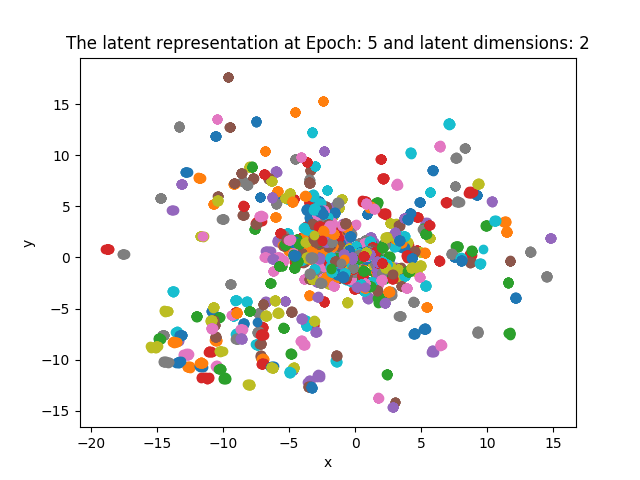
\includegraphics[width=0.23\textwidth]{../plots/task3/latent_epoch5_latent2.png} & 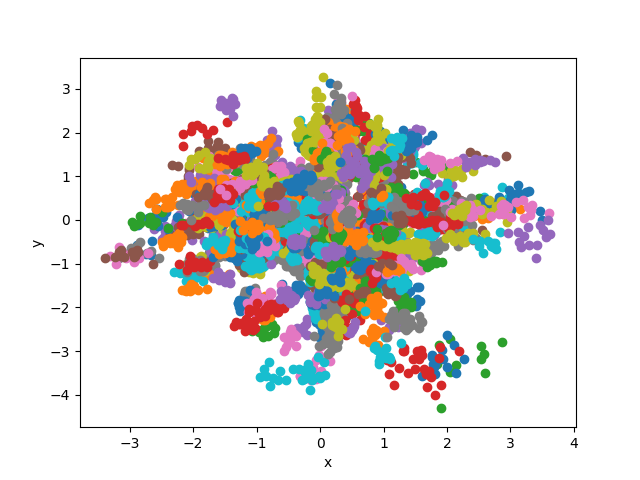
\includegraphics[width=0.23\textwidth]{../plots/task3/latent_epoch25_latent2.png} &   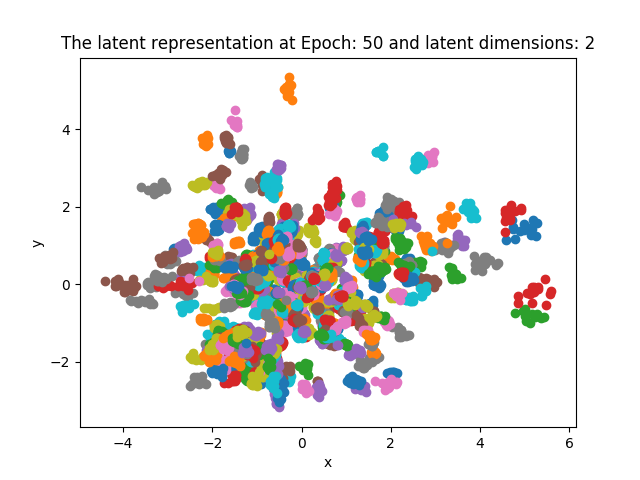
\includegraphics[width=0.23\textwidth]{../plots/task3/latent_epoch50_latent2.png} \\
      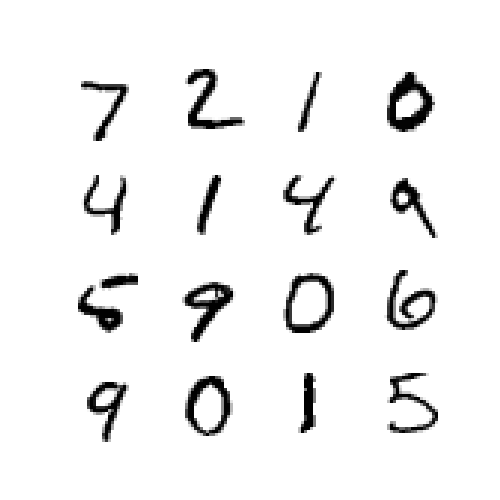
\includegraphics[width=0.23\textwidth]{../plots/task3/real_epochs1_latent2.png} &   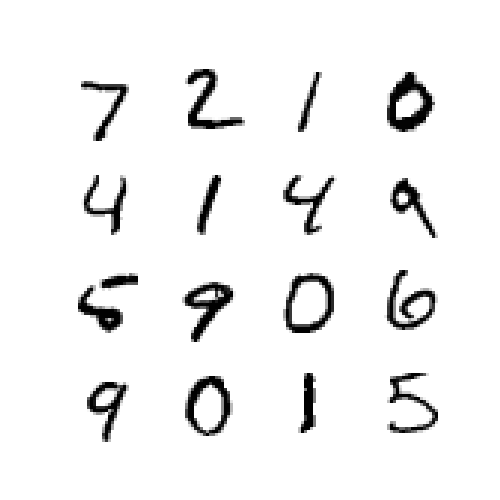
\includegraphics[width=0.23\textwidth]{../plots/task3/real_epochs5_latent2.png} & 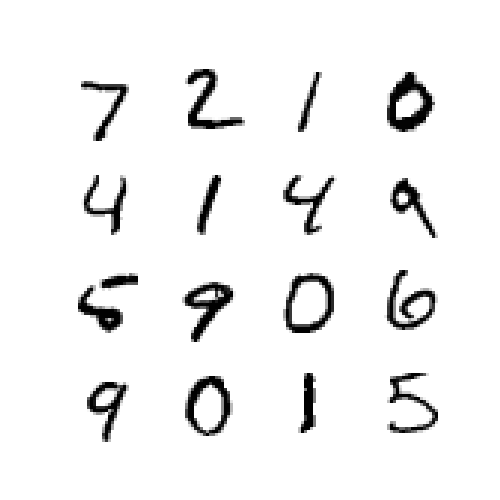
\includegraphics[width=0.23\textwidth]{../plots/task3/real_epochs25_latent2.png} &   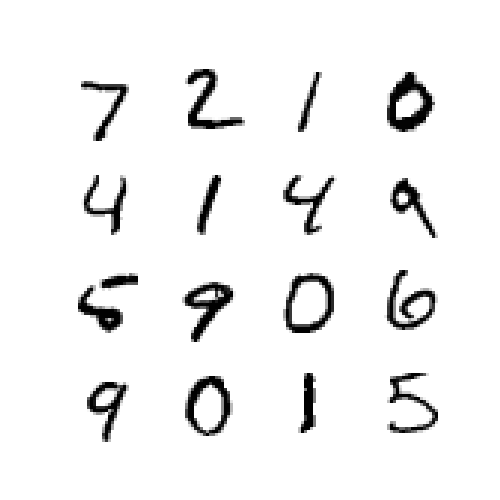
\includegraphics[width=0.23\textwidth]{../plots/task3/real_epochs50_latent2.png} \\
    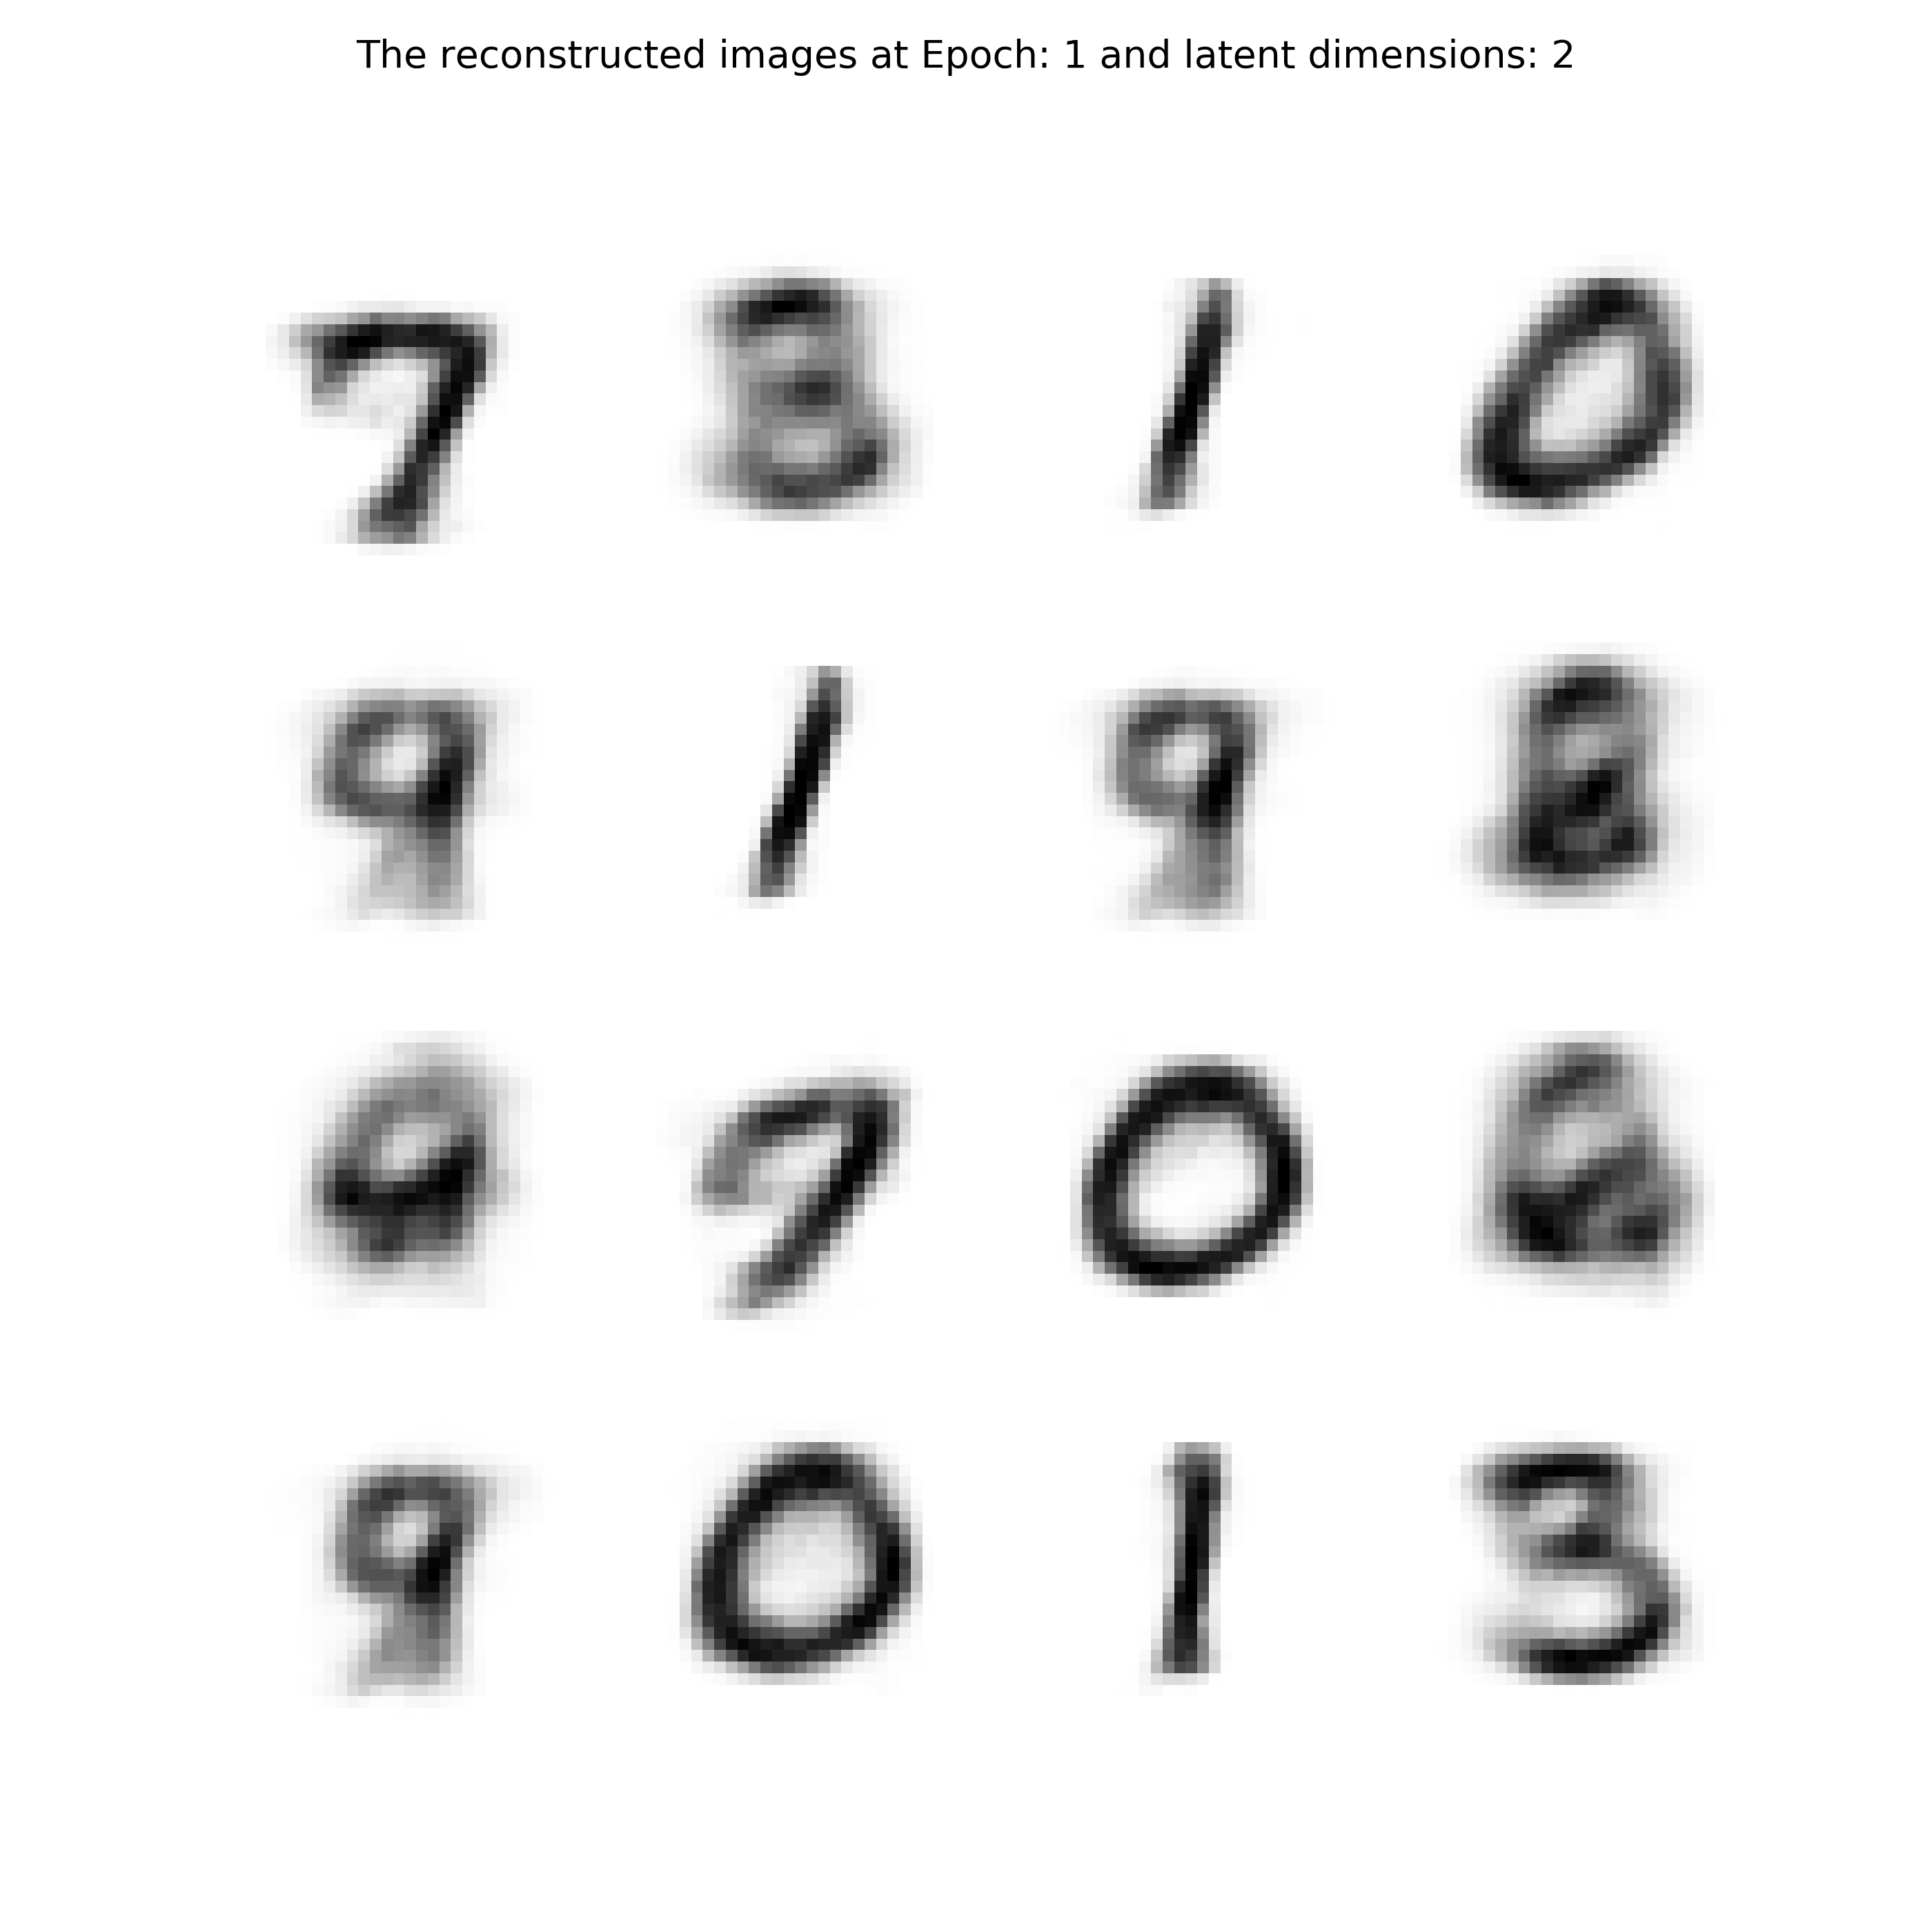
\includegraphics[width=0.23\textwidth]{../plots/task3/reconstructed_epochs1_latent2.png} &   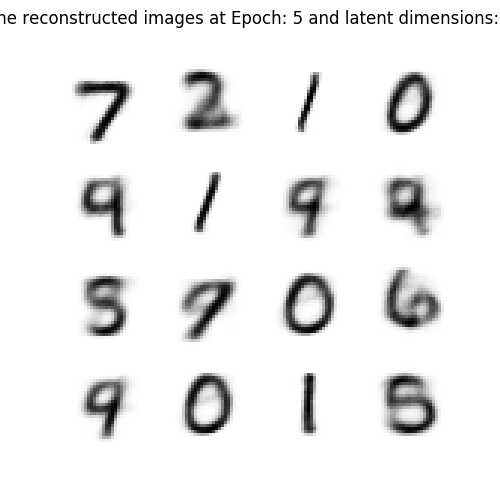
\includegraphics[width=0.23\textwidth]{../plots/task3/reconstructed_epochs5_latent2.png} & 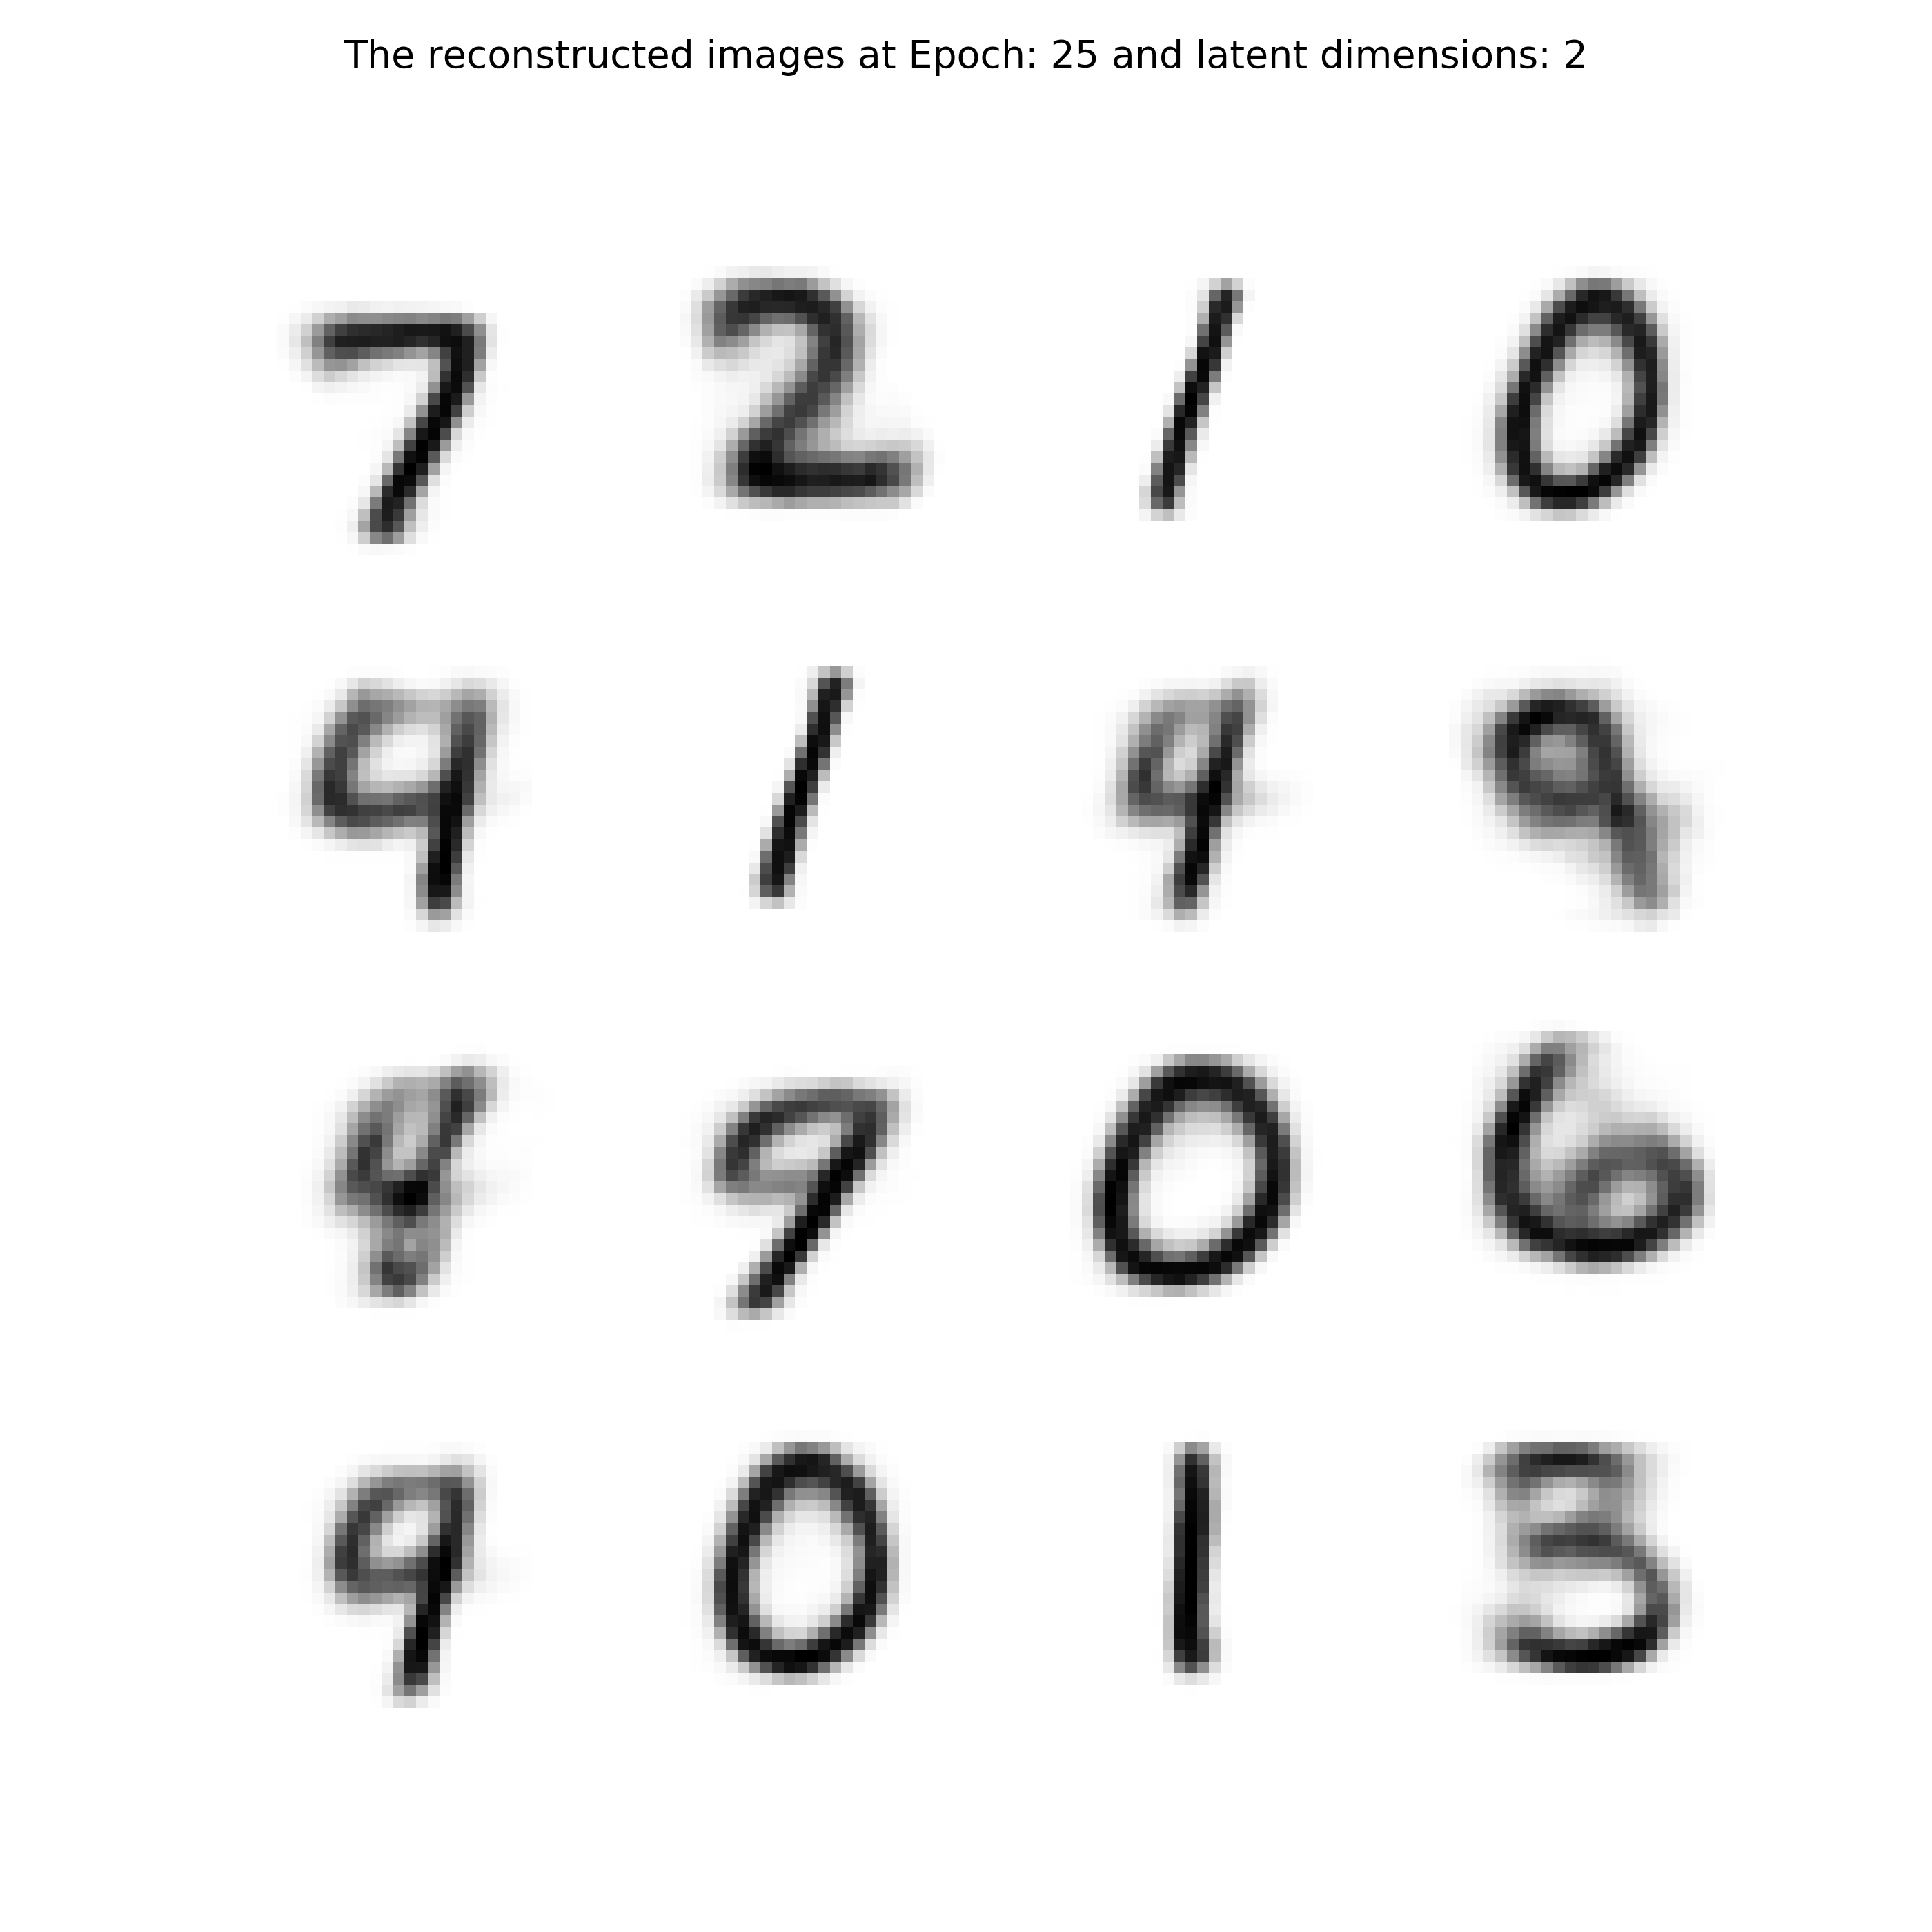
\includegraphics[width=0.23\textwidth]{../plots/task3/reconstructed_epochs25_latent2.png} &   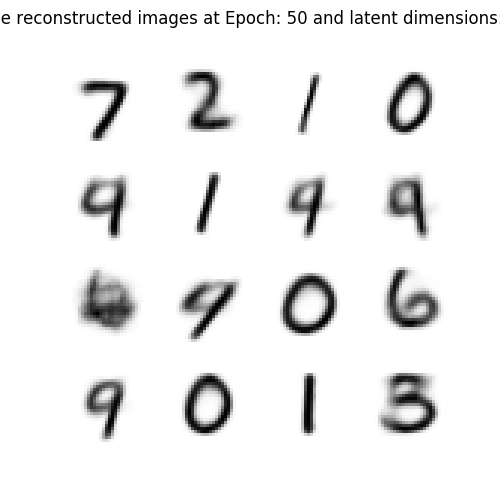
\includegraphics[width=0.23\textwidth]{../plots/task3/reconstructed_epochs50_latent2.png} \\
        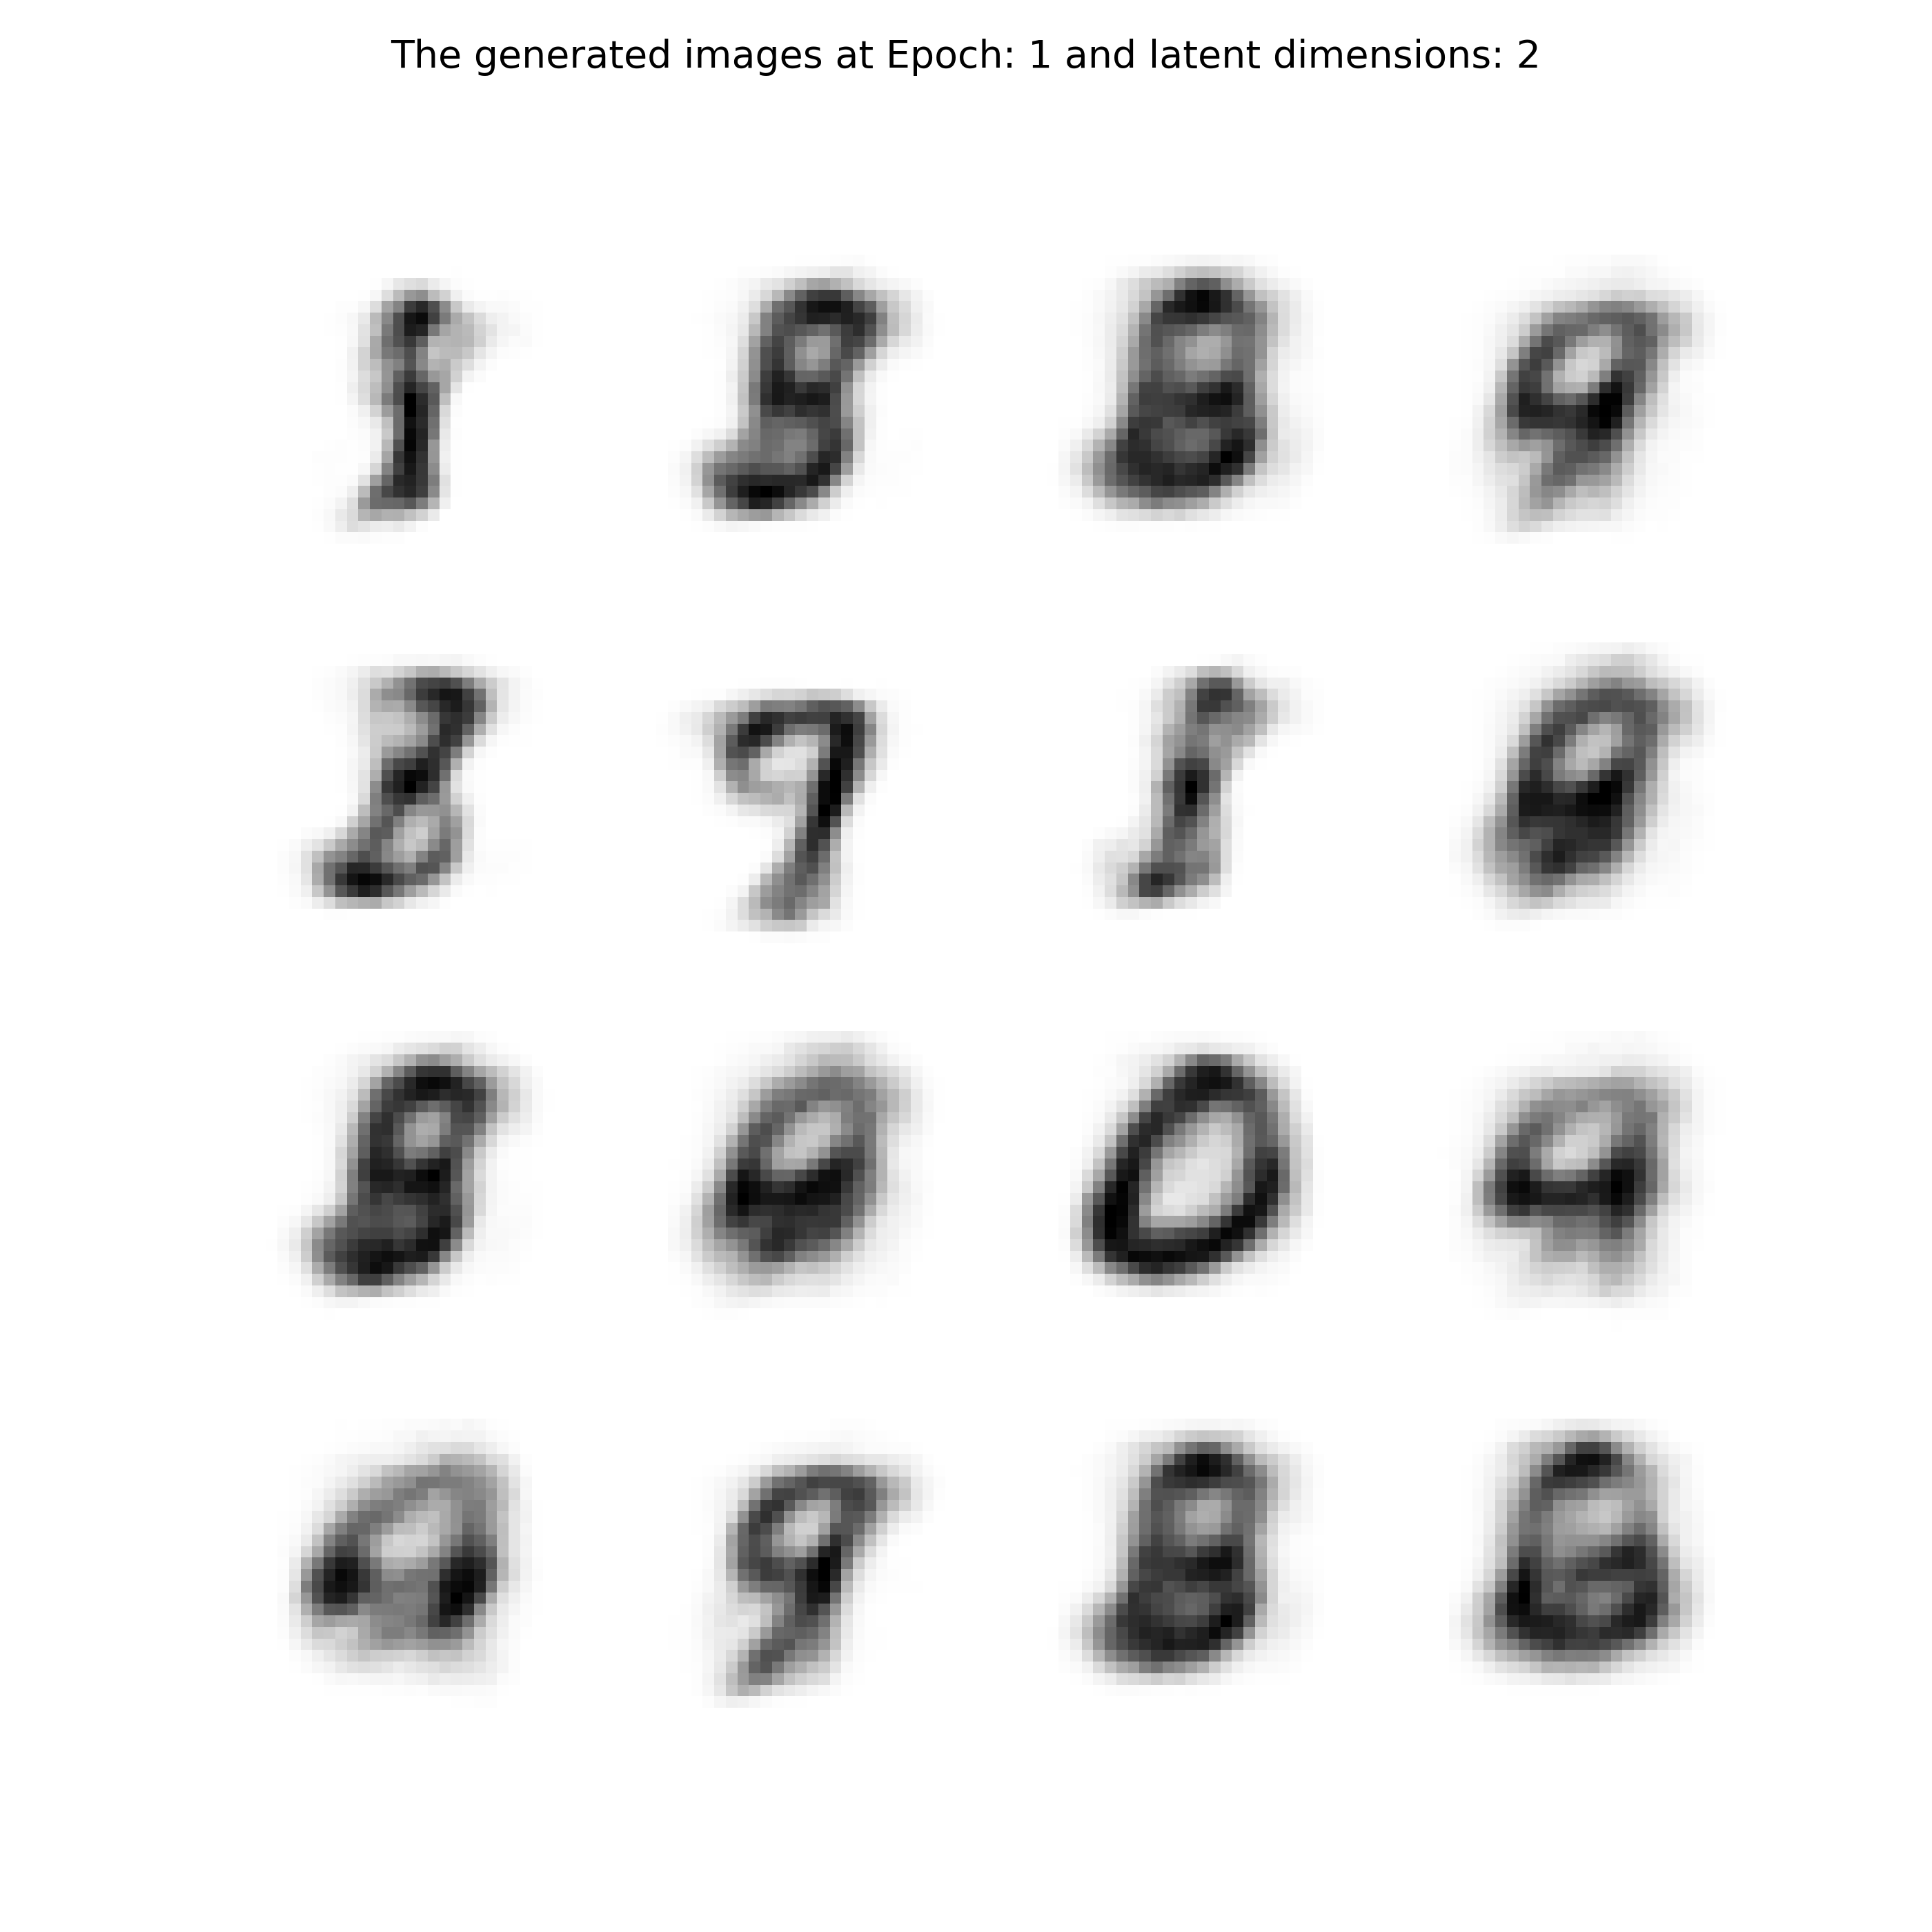
\includegraphics[width=0.23\textwidth]{../plots/task3/generated_epochs1_latent2.png} &   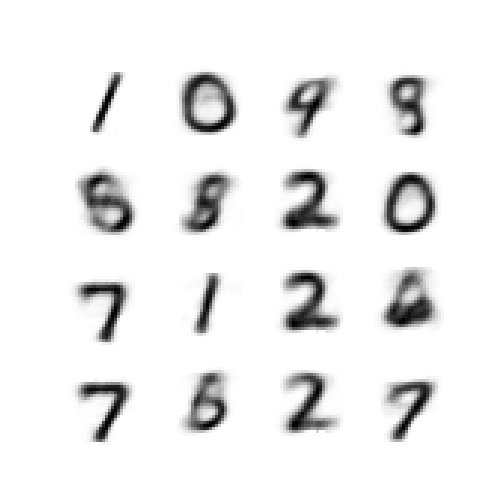
\includegraphics[width=0.23\textwidth]{../plots/task3/generated_epochs5_latent2.png} & 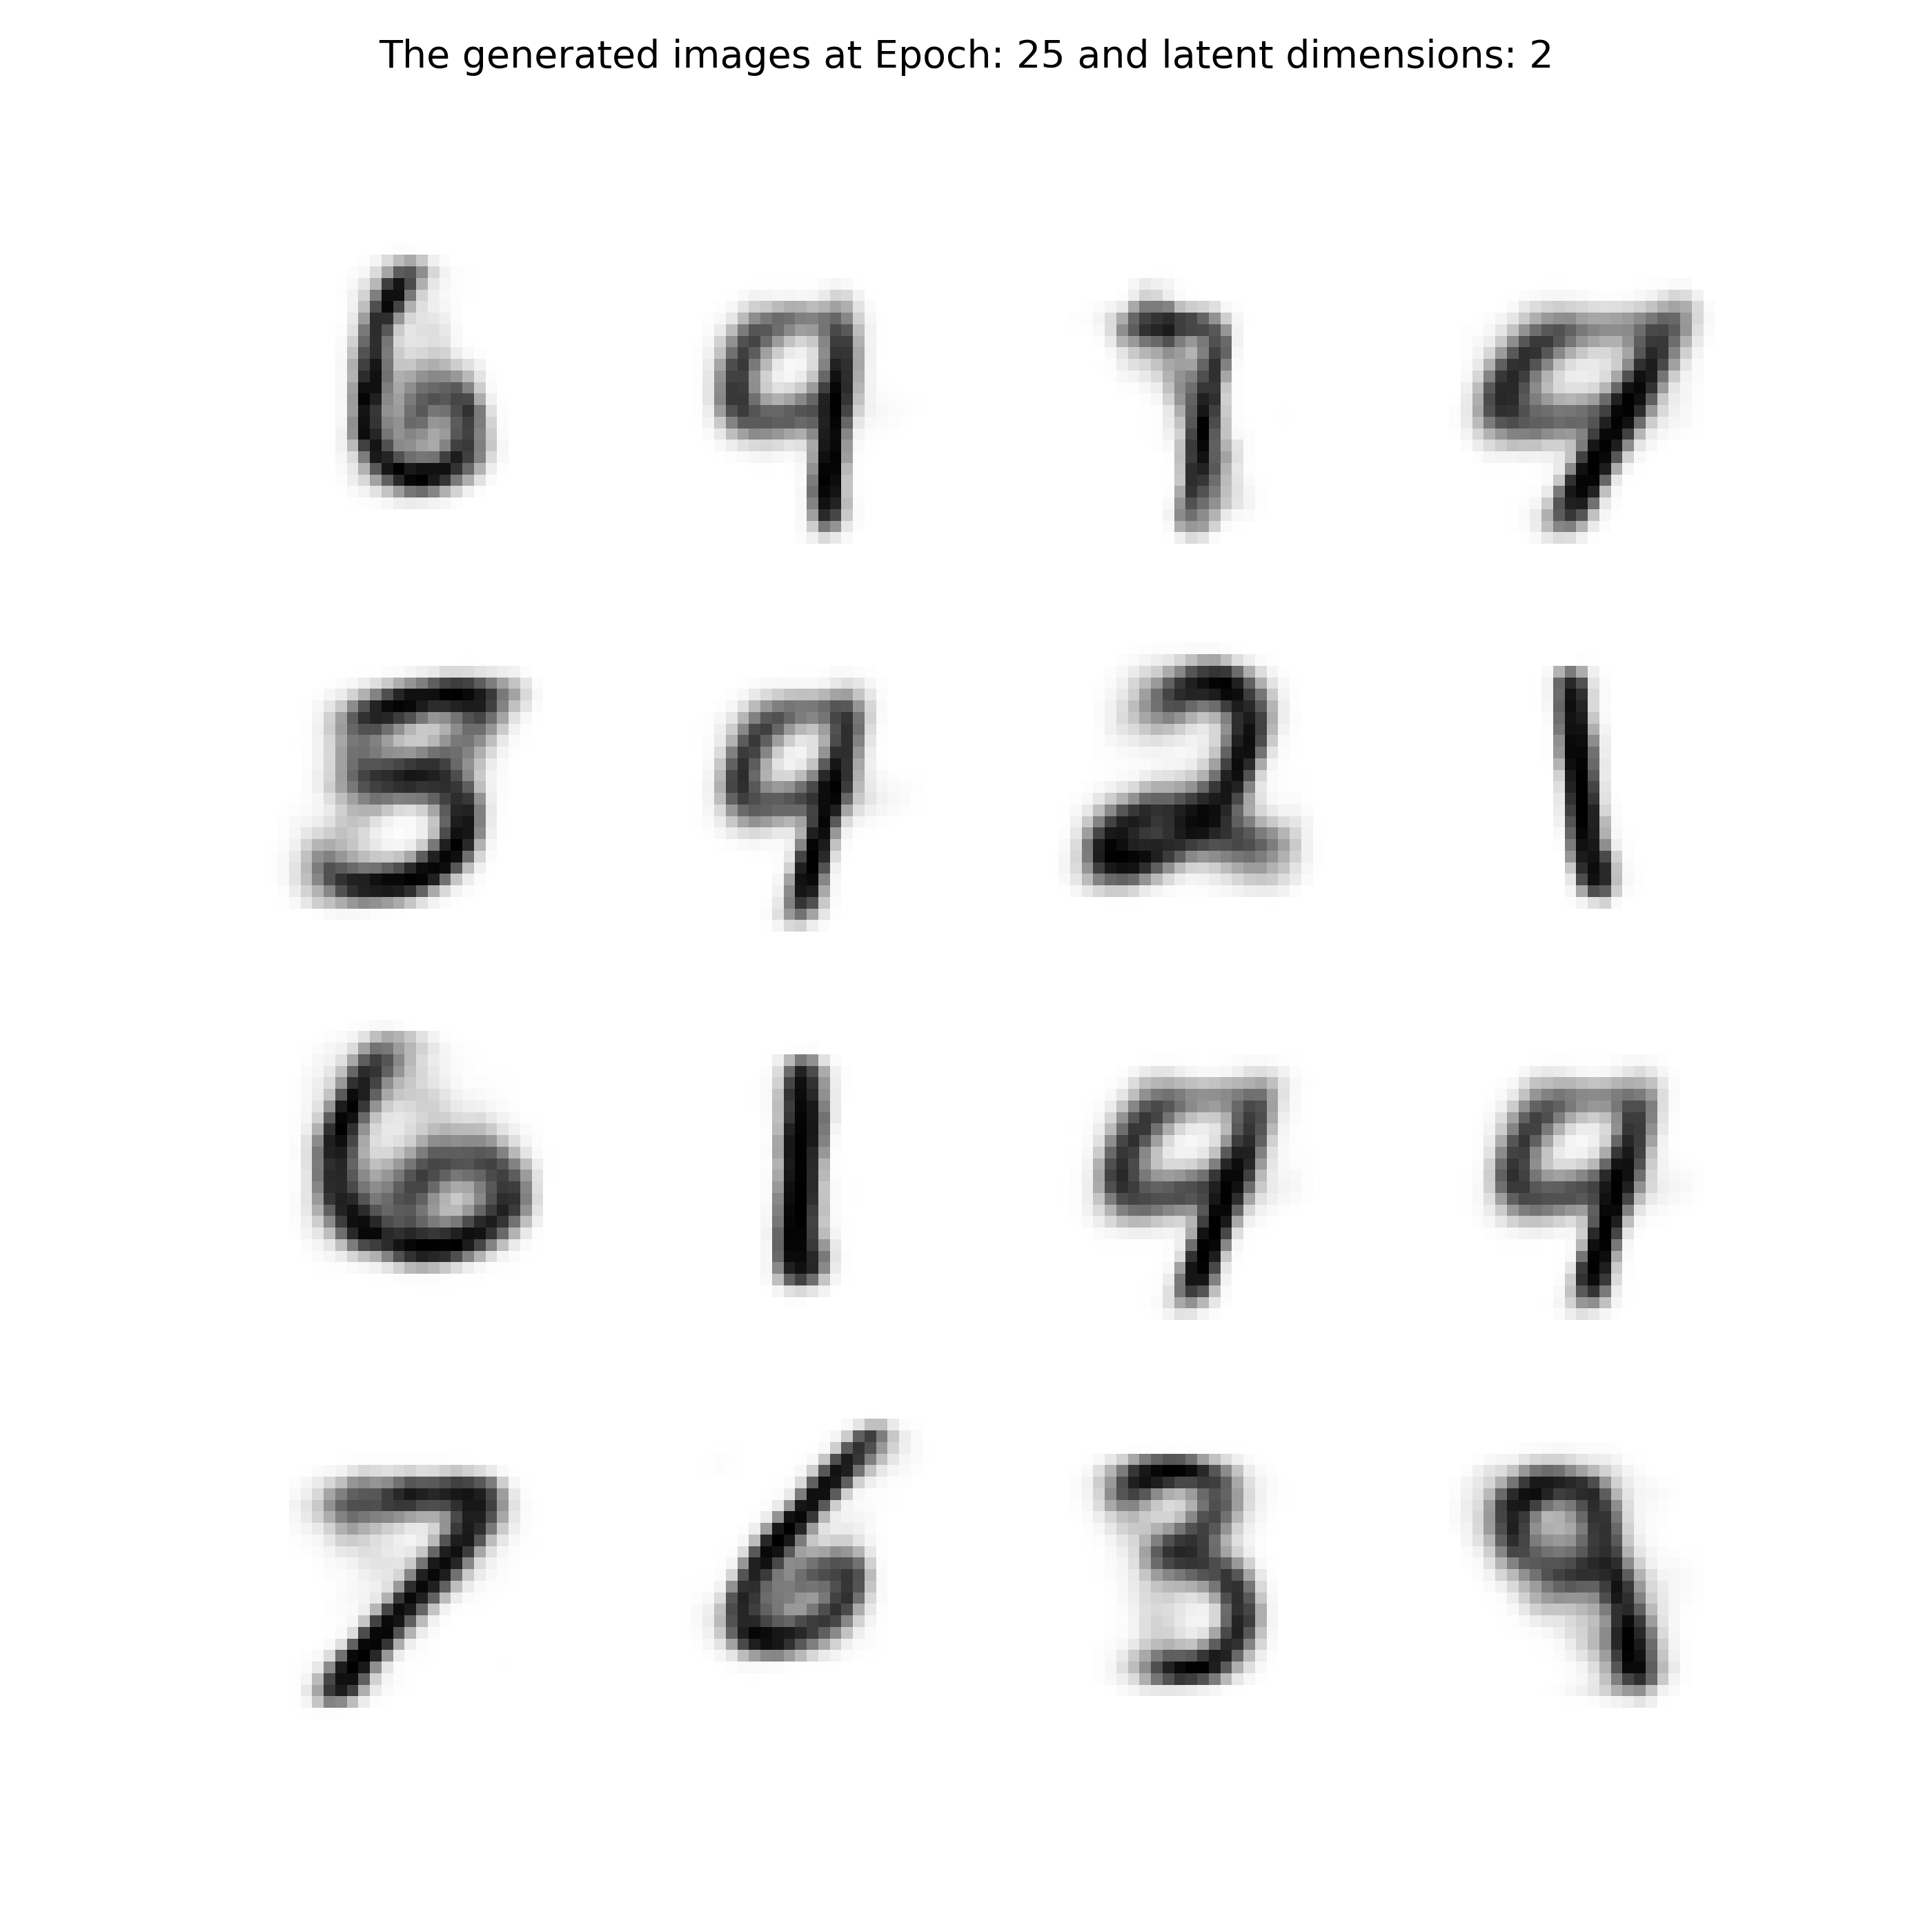
\includegraphics[width=0.23\textwidth]{../plots/task3/generated_epochs25_latent2.png} &   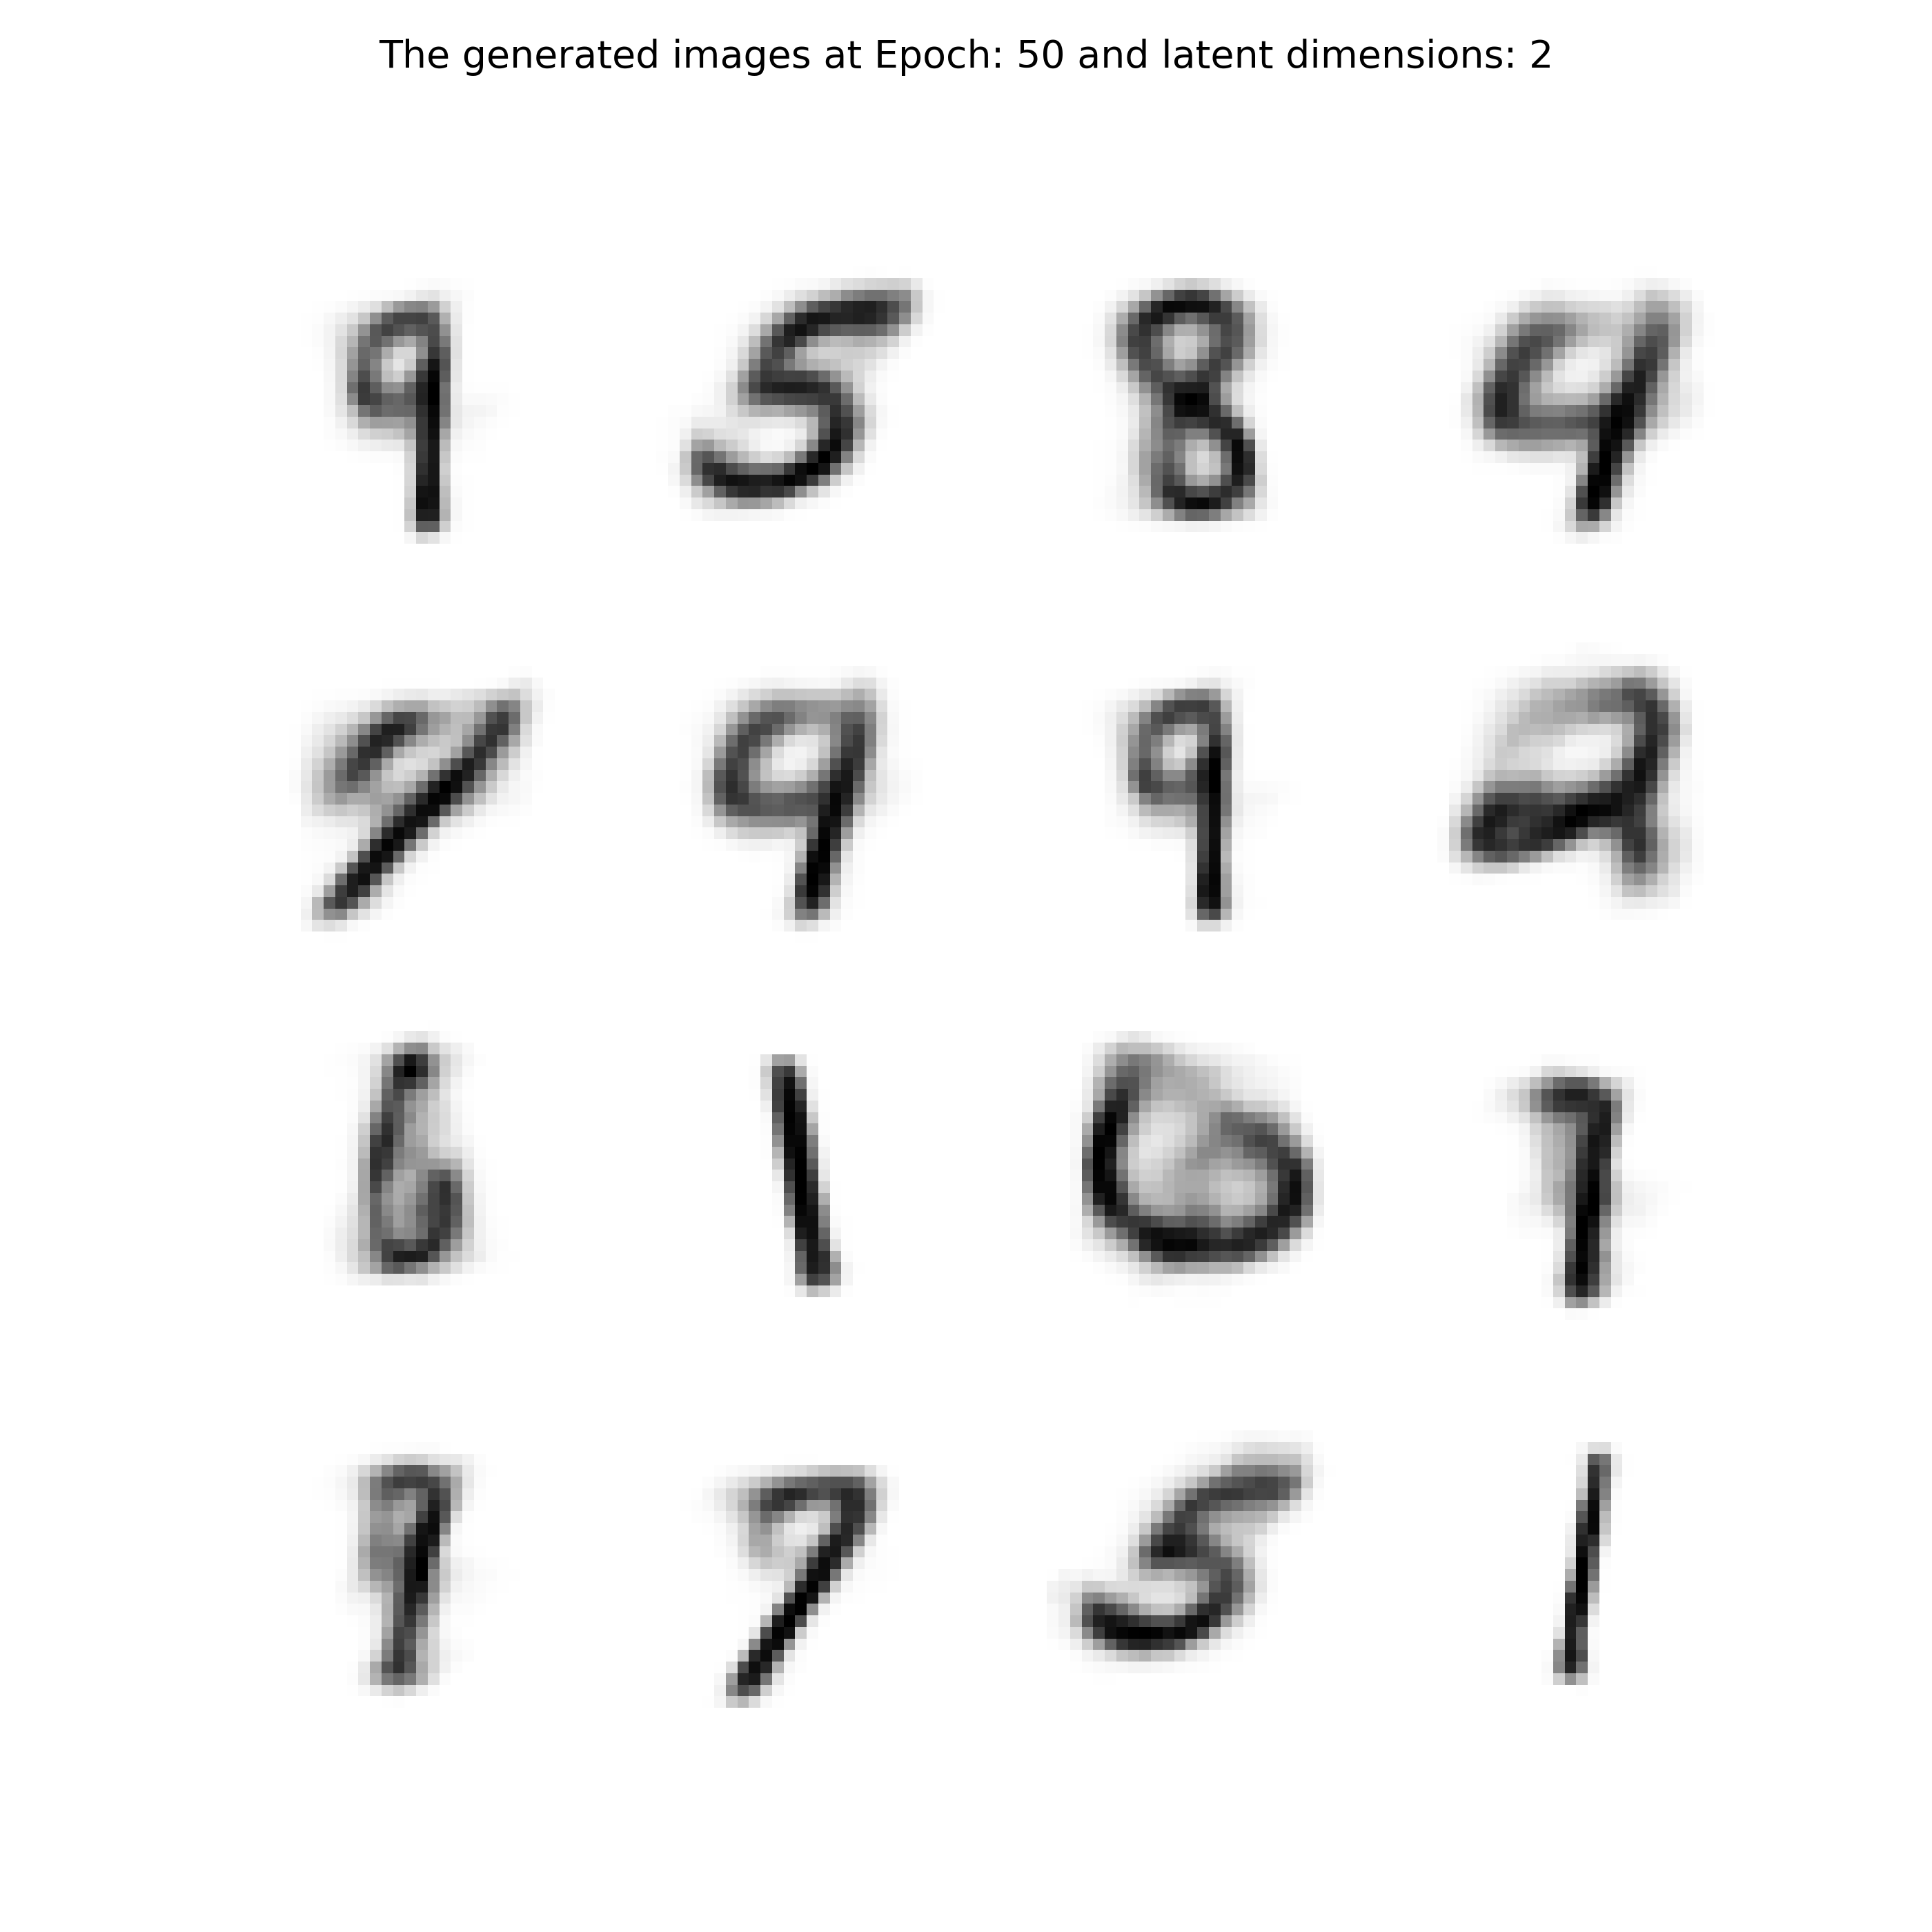
\includegraphics[width=0.23\textwidth]{../plots/task3/generated_epochs50_latent2.png} \\
\end{tabular}
\end{figure}

	\item As the VAE is trained for more epochs, the loss decreases. [\ref{fig:loss-latent-2}]
	\begin{figure}[H]
		\caption{ELBO loss}
		\label{fig:loss-latent-2}
		\centering
		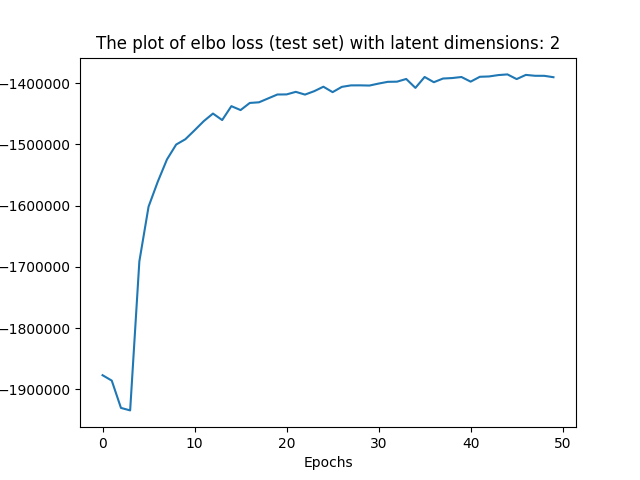
\includegraphics[width=0.45\textwidth]{../plots/task3/loss_elbo_latent2.png}
	\end{figure}	

	\item While initializing the VAE model class object, a configuration dictionary can be sent as an argument to the init function, to dynamically change the model. There are a number of configurations that can be set using the dictionary. [\ref{tab:configs_options}].
	
\begin {table}[H]
\caption {The VAE class initialization arguments} \label{tab:configs_options} 
\begin{center}
\begin{tabular}{ | m{10em} | m{20em}| } 
\hline
Argument & Description \\ 
\hline \hline
latent\_vector\_size & The dimensions of the latent vector \\ 
\hline
print\_output & Print the output plots (True or False) \\
\hline
batch\_size & Batch Size to be used \\
\hline
learning\_rate & Learning rate \\
\hline
epochs & Number of epochs\\
\hline
train\_dataloader & Pytorch dataloader for training set \\
\hline
test\_dataloader & Pytorch dataloader for test set \\
\hline
dataset\_dims & The dimensions of the dataset \\
\hline
mode & The dataset mode (mnist or mi) \\
\hline
test\_count & The number of test set data points \\
\hline
\end{tabular}
\end{center}
\end{table}

The mnist images generated using 32 dimensional latent space are more sharper. [\ref{fig:latent-32}]. The loss in this decreases more rapidly and within 50 epochs, the total loss per epoch reaches a lower value compared to the VAE trained with 2 dimensional latent space. [\ref{fig:loss-latent-32}]

\begin{figure}[H]
\caption{results obtained with a 32 dimensional latent space}
\label{fig:latent-32} 
\begin{tabular}{cccc}
	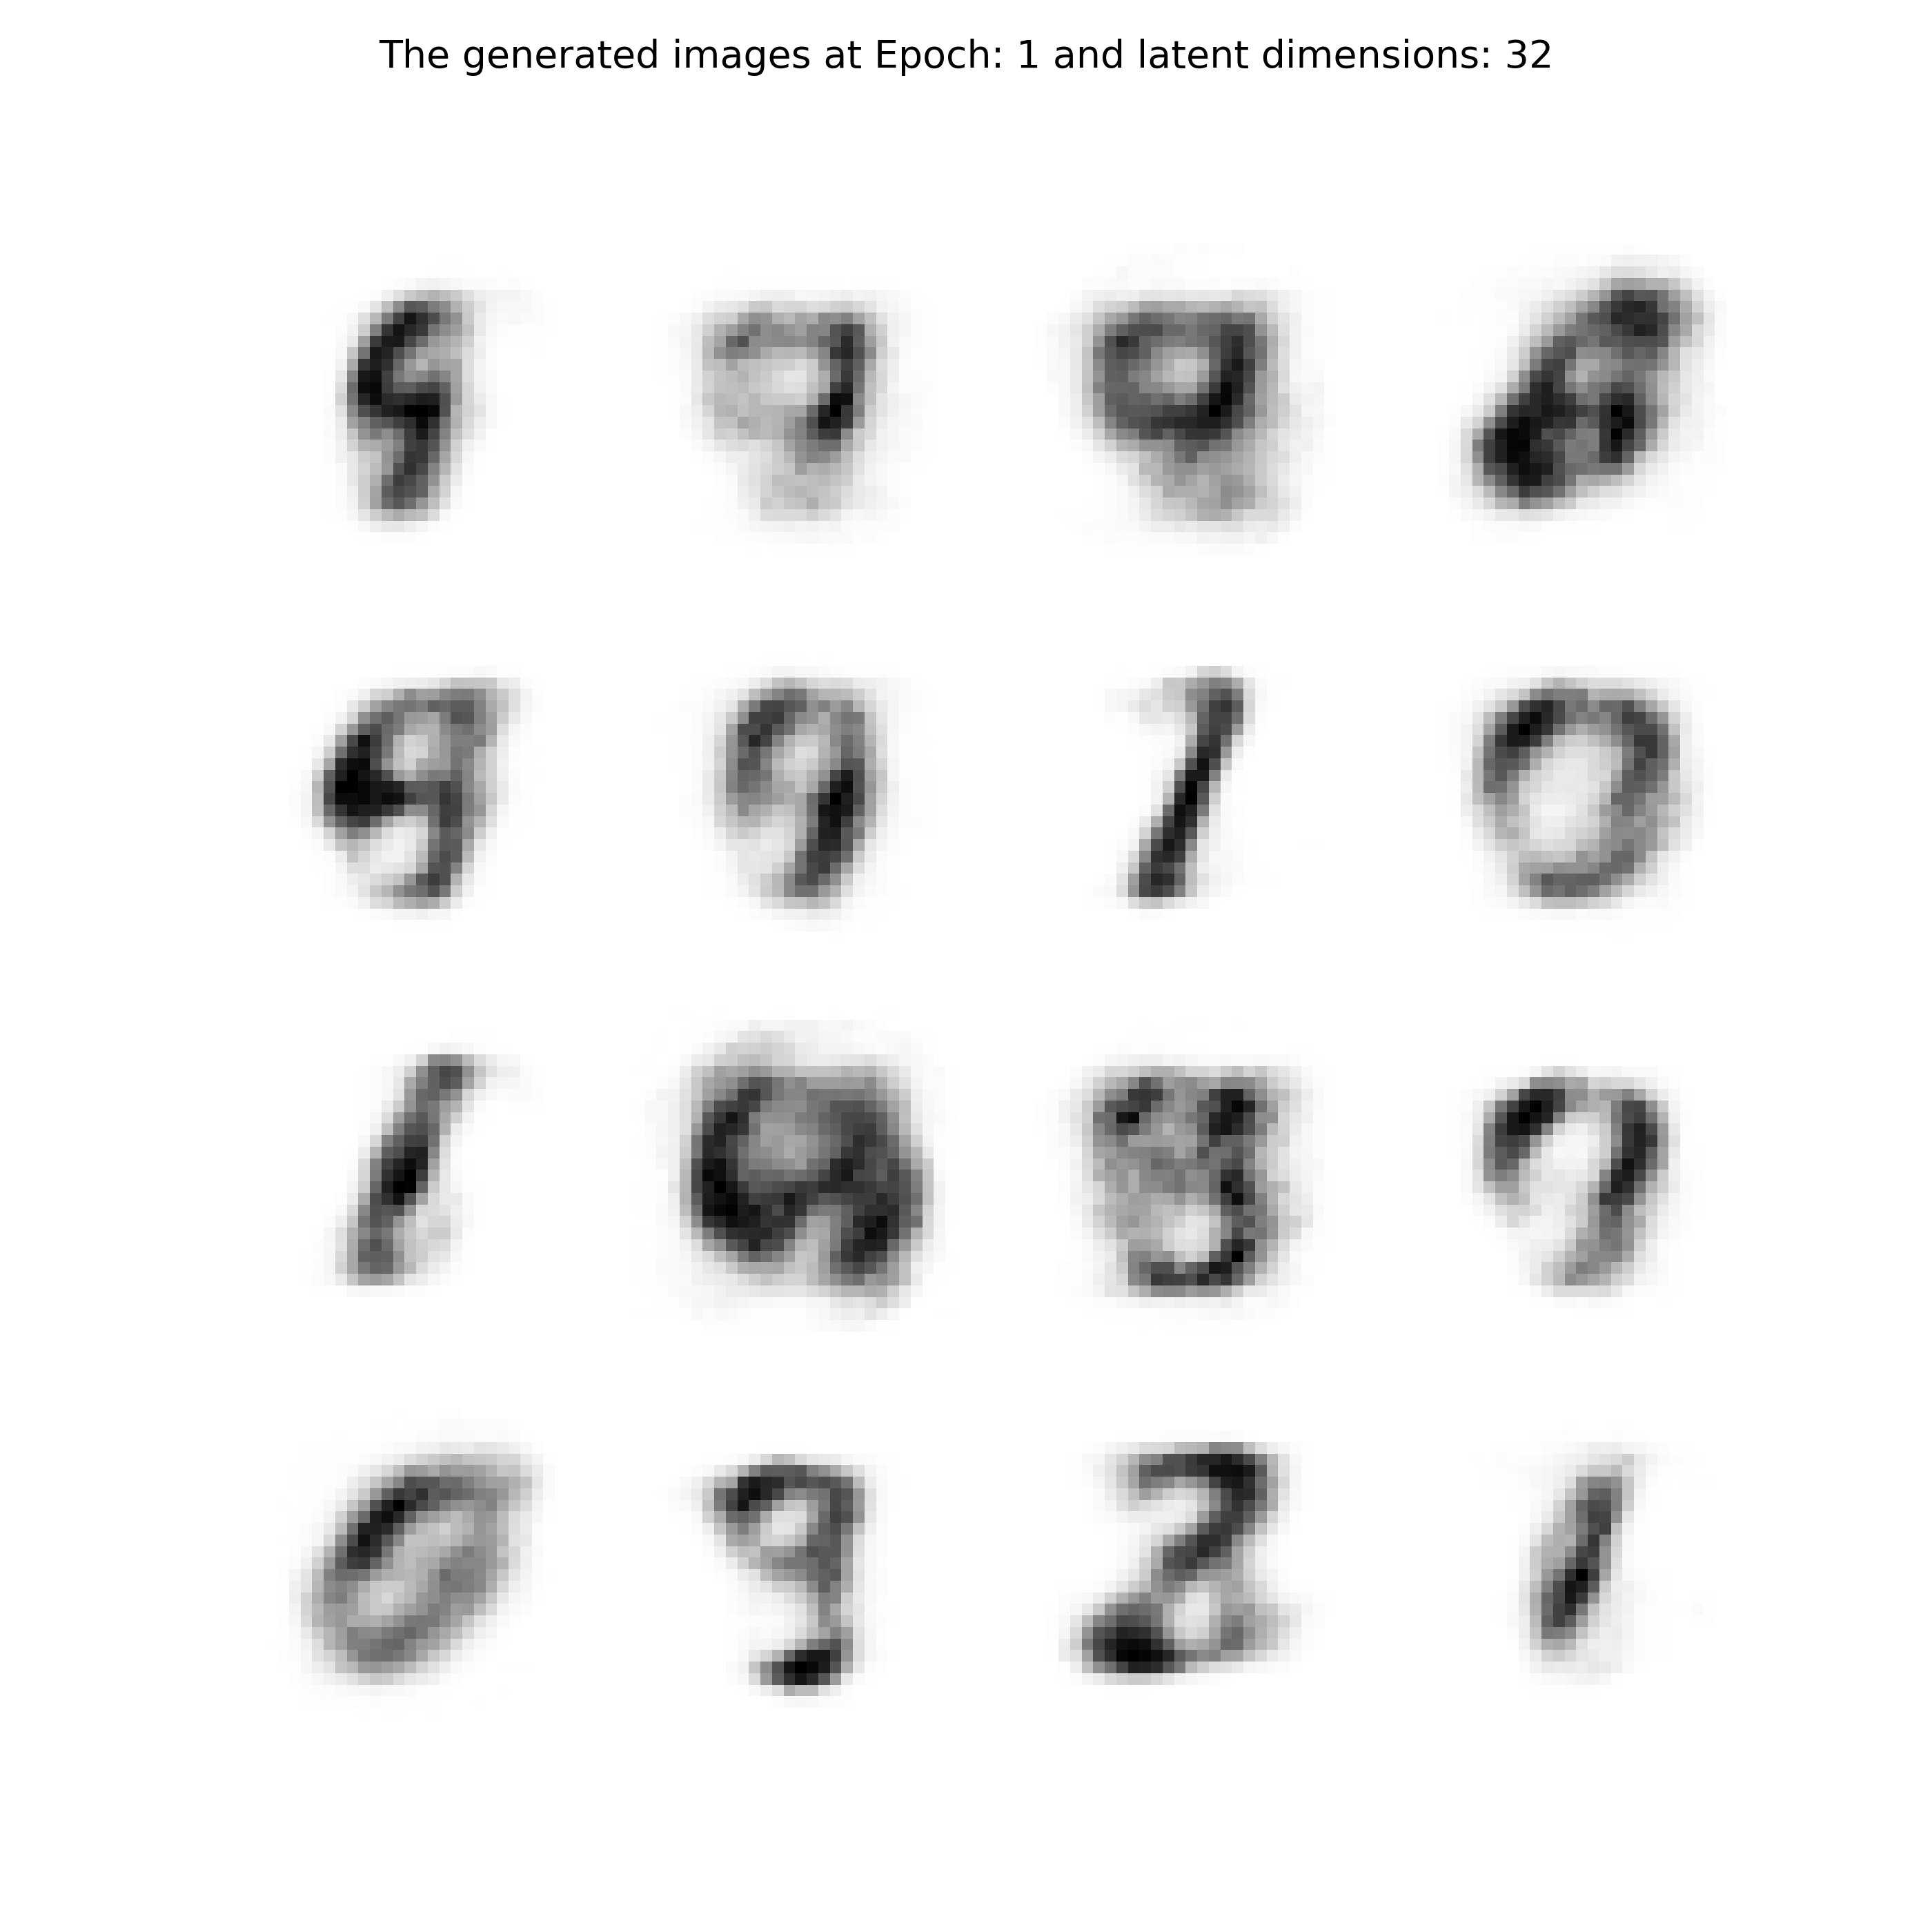
\includegraphics[width=0.23\textwidth]{../plots/task3/generated_epochs1_latent32.png} &   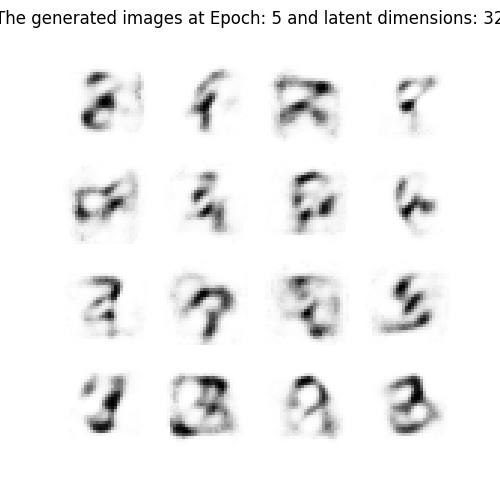
\includegraphics[width=0.23\textwidth]{../plots/task3/generated_epochs5_latent32.png} & 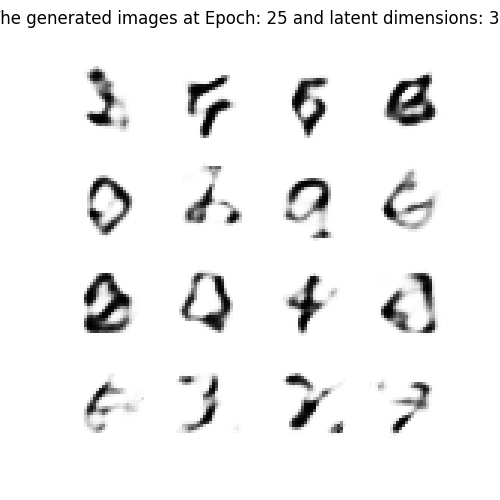
\includegraphics[width=0.23\textwidth]{../plots/task3/generated_epochs25_latent32.png} &   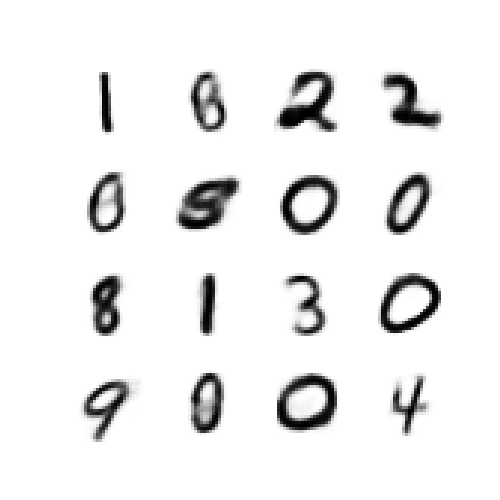
\includegraphics[width=0.23\textwidth]{../plots/task3/generated_epochs50_latent32.png} \\
\end{tabular}
\end{figure}

	\begin{figure}[H]
		\caption{ELBO loss}
		\label{fig:loss-latent-32}
		\centering
		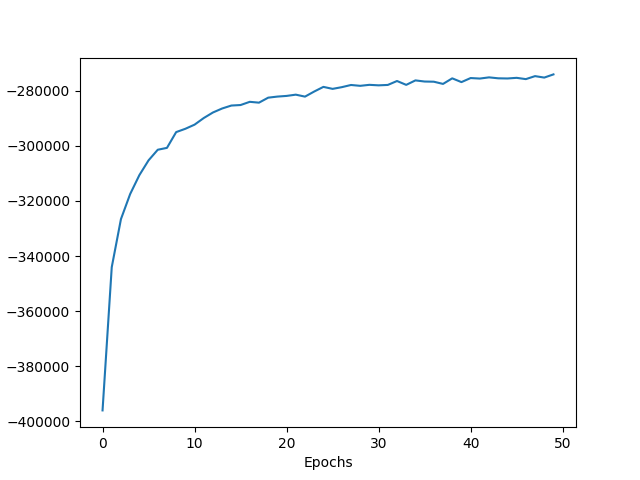
\includegraphics[width=0.45\textwidth]{../plots/task3/loss_elbo_latent32.png}
	\end{figure}

\end{enumerate}
	
\end{task}
\begin{task}{4, Fire Evacuation Planning for the MI Building}
\begin{enumerate}
	\item The training and test datasets reflect the positions of the students and employees in the campus hallways.
\begin{figure}[H]
\caption{The scatter plot of the training and test sets}
\label{fig:training-test-set} 
\begin{tabular}{cc}
	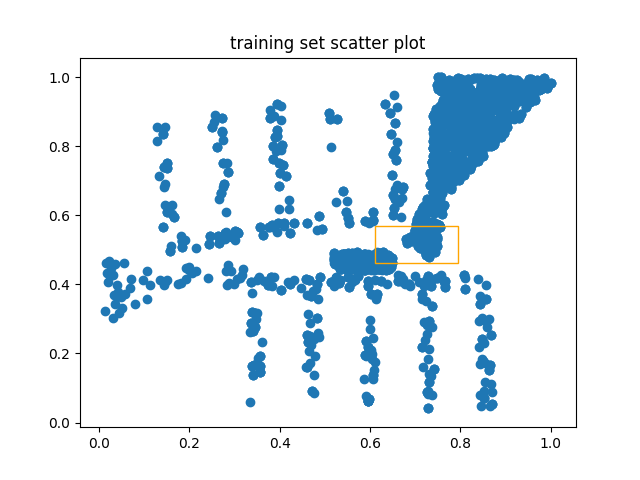
\includegraphics[width=0.45\textwidth]{../plots/task4/training_set_scatter.png} &   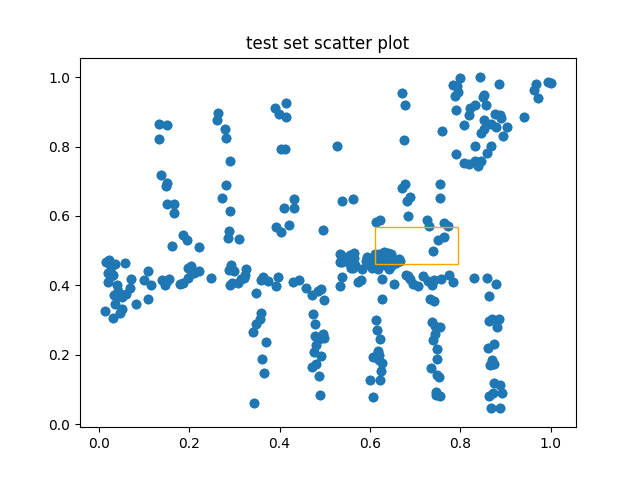
\includegraphics[width=0.45\textwidth]{../plots/task4/test_set_scatter.png} 
\end{tabular}
\end{figure}
	\item The same VAE implementation is used for training a VAE on the FireEvac data. The 'mode' argument is set to mi and the 'dataset\_dims' argument is set to 2, as the FireEvac dataset is 2 dimensional. A number of modifications have to be made to train the FireEvac dataset:
	\begin{itemize}
		\item The VAE is trained for 1000 epochs. 
		\item The learning rate of the adam optimizer is set to 0.0001 because the higher learning rate of 0.001 used in the previous task proves to be too high for training the FireEvac data. It results in a jittery model training.
		\item Mean Squared Error is used for calculating the reconstruction loss. The predicted data is the output of the decoder and the target is the input data.
		\item Relu activation function is used for the last layer of decoder, as the FireEvac data consists of positive unbounded coordinates.
	\end{itemize}
	
	\item The distribution of the data reconstructed from test set, is similar to test set distribution. [\ref{fig:reconstructed-data}]
	\begin{figure}[H]
		\caption{ELBO loss}
		\label{fig:reconstructed-data}
		\centering
		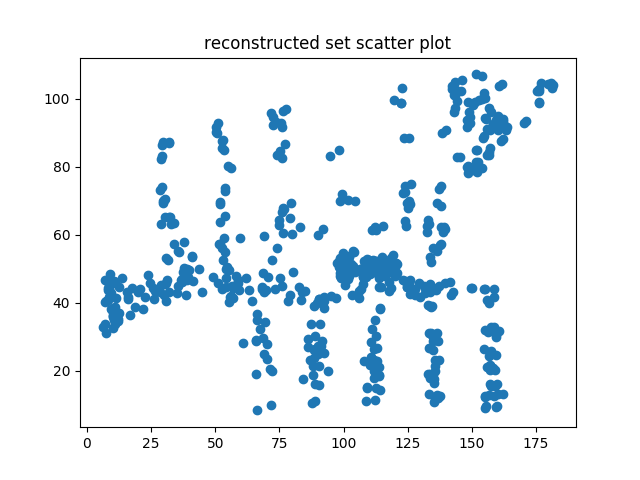
\includegraphics[width=0.45\textwidth]{../plots/task4/reconstructed_set_scatter.png}
	\end{figure}
\end{enumerate}
\end{task}
\end{document}
